\begin{refsection}
%-------------------------------------------------------------------------
%-------------------------------------------------------------------------
\chapter{X-rays as a branch of optics}\label{sec:x-ray_optics}
%-------------------------------------------------------------------------
%-------------------------------------------------------------------------

In the late 1920s, not much longer after their discovery in late 1895, X-rays were already consolidated as a branch of optics. This chapter opens up with a brief recount of the early days of X-ray optics and main focusing optical element families. The compound refractive lenses (CRLs), the main topic of this work, are then presented at length and the modelling of ideal CRLs accounting their thick-element nature is derived. Some figures of merit for their optical performance are also discussed.

%-------------------------------------------------------------------------
%-------------------------------------------------------------------------
\section{The early days of X-ray optics}\label{sec:early_days}
%-------------------------------------------------------------------------
%-------------------------------------------------------------------------

Upon reporting the discovery of  X-rays in [\cite{Roentgen1896_ch3}], R\"{o}ntgen describes several properties, among them: a) that refraction cannot be conclusively observed and if the tested materials\footnote{The materials used were water, carbon disulfide, mica, ebonite and aluminium.} do refract the X-rays, their index of refraction cannot be larger than 1.05 [cf. \textit{§7} ibid.]; b) there is no noticeable regular reflection of the rays on none of the substances\footnote{Platinum, lead, zinc and aluminium.} examined [cf. \textit{§8} ibid.]; c) there is no observable interference phenomena [cf. \textit{§15} ibid.]; d) and finally, that the X-rays cannot be polarised\footnote{In fact, this observation is not accompanied by any experimental observation described in his manuscript, but it comes from him speculating about the X-rays nature: \textit{"If one asks oneself what the X-rays [...] actually are [...]. If the X-rays were to be ultraviolet light, this light should have the property: [...] c)
that it cannot be polarised by the usual means;"} [\cite[\textit{§17}]{Roentgen1896_ch3}].} by the usual means [cf. \textit{§17c} ibid.]. At the time of the discovery of the X-rays, their only likeness to light was that they propagated in a straight line in free-space. It took about 30 years for this to change.

Between the years of 1904 and 1906 polarisation in X-rays has been described and observed by C. Barkla [\cite{Barkla1904, Barkla1905, Barkla1906}]. Speculations and experiments regarding diffraction of X-rays start as early as the 1900s [\cite{Haga1903,Walter1908,Walter1909}], but it was not until the early 1910s that diffraction was successfully described [\cite{Laue1912}], observed [\cite{FriedrichKnippingLaue1912}] and modelled by what came to be known as the Bragg law of refraction [\cite{BraggW.H.1913}]. Early experiments aiming direct observation of refraction failed, but helped narrowing the index of refraction for the X-ray regime\footnote{C. Barkla's experiment aimed to measure the refractive index of potassium bromide for radiation of wavelength in the neighbourhood of 0.5~\r{A}.} to $0.999995\leq n \leq1.000005$ [\cite{Barkla1916}]. Further experimental observations of Bragg's law started showing small deviations between expected and obtained values. These were first reported by \citeauthor{Stenstrom1919} in \cite*{Stenstrom1919}\footnote{The same kind of discrepancies were also observed and reported by \citeauthor{Duane1920} in \cite*{Duane1920} and \citeauthor{Siegbahn1920} in \cite*{Siegbahn1920} and \cite*{Siegbahn1921}.} and were attributed to the refraction of the X-rays as they penetrate the crystal\footnote{This was met by criticism from \citeauthor{Knipping1920} in \cite*{Knipping1920} \citep{Knipping1920}. However, as pointed out by A. \citeauthor{Compton1923} - cf. [\cite{Compton1923}], theoretical calculations made by \citeauthor{Ewald1920} in \cite*{Ewald1920} showed good agreement between experimental observations and the refraction hypothesis [\cite{Ewald1920}].}, limiting the index of refraction to $n\lesssim1$ [\cite[\textit{§3}]{Stenstrom1919}]. The experimental proof of the refraction of X-rays came in the mid-1920s with [\cite{Larsson1924}]. Being able to detect refraction was very important, as it directly allows to assume the existence of reflection which
can only occur if in a boundary surface there is a discontinuity in the indexes of refraction between the two media. If one of these phenomena is present, the the other one must too exist [\cite{Compton1928}]. Based on earlier reports about the discrepancies observed on the Bragg's law of refraction, A. \citeauthor{Compton1923} was able to estimate the glancing angles for polished surfaces of several materials and demonstrate the total external reflection of X-rays [\cite{Compton1923,Prins1927}]. In fact, by the end of the 1920s, all fundamental characteristics\footnote{Reflection, refraction, diffraction, polarisation, diffuse scattering, emission and absorption spectra and the photoelectric effect are the essential characteristics of light considered by A. Compton in [\cite{Compton1928}].} of light have been found to be present for X-rays, making them undoubtedly a branch of optics [\cite{Compton1928}].  

%-------------------------------------------------------------------------
%-------------------------------------------------------------------------
\subsection{X-ray focusing optics}
%-------------------------------------------------------------------------
%-------------------------------------------------------------------------

Parallel to the early observation of the phenomena that showed that X-rays are a branch of optics, came the development of optical elements exploiting diffraction, reflection and refraction for focusing of X-rays\footnote{This recount of the early days of X-ray focusing optics is oriented to accelerator-based X-rays. The field of X-ray optics for astronomy is very rich, but is not covered here, but a review is available in [\cite{Gorenstein2010}].}.

%-------------------------------------------------------------------------
%-------------------------------------------------------------------------
\subsubsection*{Diffractive optics}\addcontentsline{toc}{subsubsection}{-- Diffractive optics}
%-------------------------------------------------------------------------
%-------------------------------------------------------------------------

The early optical elements based on diffraction for focusing of X-rays were curved crystals operating on the Bragg diffraction condition [\cite{Gouy1916,Seemann1916}]. The use of curved crystals\footnote{Several early works on curved crystals often refer to "systems operating on Bragg reflection", which is actually an euphemism for diffraction.} for focusing X-rays came in context of optimising the performance of spectrographs (spectrometers) with major contributions from [\cite{Johansson1933,V.Hamos1933, Hamos1937}]. Other historical milestones are multi-layer mirrors\footnote{In the multi-layer mirrors it is not the total external reflection effect that reflects the X-rays, but Bragg diffraction from the periodic arrangement of the layered structture on the mirror surface.}, monochromators [\cite{Smith1941}] and gratings monochromators [\cite{refMonoGrating}] and zone-plates\footnote{Often referred to X-ray lenses up until the ealy 1990s, when refractive X-ray lenses were demonstrated for the first time [\cite{Snigirev1996}].} [\cite{Baez1960,Schmahl1969,Kirz1974}]. More recent developments include (multi-layer) Laue lenses [\cite{refMLL}], kinoform lenses\footnote{Kinoform lenses are a hybrid between diffractive- and refractive optics [\cite{Jordan1970}].} [\cite{refKino}] and diffractive corrective optics for focusing elements [\cite{Probst2020}].


%-------------------------------------------------------------------------
%-------------------------------------------------------------------------
\subsubsection*{Reflective optics}\addcontentsline{toc}{subsubsection}{-- Reflective optics}
%-------------------------------------------------------------------------
%-------------------------------------------------------------------------

Using total external reflection for focusing X-rays started around the late 1940s with [\cite{Ehrenberg1947, Kirkpatrick1948, Ehrenberg1949, Kirkpatrick1950}] in the context of direct imaging and X-ray microscopy\footnote{Early works on "X-ray microscopy" are based on imaging of the reciprocal space with the necessity of Fourier transformations to recover the image in the direct space [\cite{Bragg1939,Bragg1942}].}, moving away from the spectroscopy application of the previous decades. Soon after several X-ray mirror designs emerged [\cite{Wolter1952,Montel1957}] and continue to do so today [\cite{refNewMirrors}]. X-ray mirrors have a very wide use in X-ray optics and a general review can be found in [\cite{Howells1993,Susini1993}].

%-------------------------------------------------------------------------
%-------------------------------------------------------------------------
\subsubsection*{Refractive optics}\addcontentsline{toc}{subsubsection}{-- Refractive optics}
%-------------------------------------------------------------------------
%-------------------------------------------------------------------------

Finally, the group of optical elements based on refraction of X-rays for focusing light should be presented. Refractive X-ray optics comprises mainly lenses [\cite{Snigirev1996}], prisms in several arrangements [\cite{Cederstrom2000, Jark2004}] and most recently, free-form objects mainly for optical correction and beam-shaping [\cite{Seiboth2017, Zverev2017, Seiboth2019, Seiboth2020, Dhamgaye2020}]. From those, compound refractive lenses (CRLs) - as X-ray lenses are called - are by far the dominating refractive optical element in use throughout synchrotrons. In retrospective, they are the least mature, dating from the mid-1990s, while the use of diffractive focusing optics dates to the early 1930s and reflective optics to the late 1940s. 


%-------------------------------------------------------------------------
%-------------------------------------------------------------------------
\subsubsection*{- A bit of history\footnote{This was originally published as \textit{§3.1~-~Prelude} in [\cite{Celestre2017}].}}
%-------------------------------------------------------------------------
%-------------------------------------------------------------------------
X-ray lenses were long believed to be unfeasible: low refraction index leads to unpractical focal lengths and the transmission of X-rays through matter faces strong absorption. In one of the early works on focusing and imaging with X-ray optics, P. Kirkpatrick and A. Baez stated that: \textit{"about one hundred lens surfaces in series would be required to bring the focal length down to one hundred meters. This would produce a cumbersome and very weak lens system of poor transparency. These discouraging considerations incline us toward other methods"}\footnote{Using $f=R/\delta$, where $f$ is the focal length and $R$ is the refractive surface radius (cf. Eq~\ref{eq:Focus_simple}). The estimation shows values for $R=1$cm, using beryllium lens at $\lambda=0.71$\r{A}, K$_{\alpha}$ line of molybdenum \cite{Kirkpatrick1948}.} [\cite{Kirkpatrick1948}]. On the following year, Kirkpatrick went on to say: \textit{"Although the X-ray lens is thus possible it has the disadvantages of high absorption and strong chromatic aberration, and so would probably be generally inferior to mirror systems"} [\cite{Kirkpatrick1949}]. 

It was not before 1991 that X-ray lenses would be reconsidered: in a scientific correspondence to the journal Nature, a Japanese group headed by S. Suehiro proposed the use of such elements for the forthcoming third generation light sources [\cite{Suehiro1991}]. Such idea was not met with enthusiasm by the X-ray optics community, who still considered such technologies to be impractical for focusing X-rays as it was made clear by A. Michette, who had written Nature a reply to Suehiro's communication. The text entitled \textit{"No X-ray lens"} criticises the idea of refractive optics for X-rays and lists the reasons why those were considered them unsuitable for focusing X-rays [\cite{Michette1991}]. In \textit{"Fresnel and refractive lenses for X-rays"} by B. X. Yang, written in 1992 and published in 1993, Yang revisited S. Suehiro's idea and proposed ways to overcome the strong absorption of such lenses by using a Fresnel lenses shape instead [\cite{Yang1993}], however those were at the time of complicated fabrication and were not given too much attention. 

The birth of the X-ray refractive lens as known today can be traced back to 1994, when T. Tomie filed a patent for X-ray lenses in Japan [\cite{Tomie1994}] - patents were also filed in US and Germany on the following year. His concept for X-ray lenses was introduced to the scientific community as poster on the \textit{XRM'96, Int. Conf. X-ray Microscopy and Spectroscopy}, held in W\"urzburg, Germany, in 1996. The concept was simple, but innovative: a series of drilled holes into a single substrate along a straight line. The proposed design increased mechanical robustness, overcame alignment issues, reduced absorption by placing the drilled holes close to each other and was relatively simple to be manufactured - although T. Tomie never went on to produce them [\cite{Tomie2010}]. Shortly after the presentation of the refractive lens to the scientific community at the XRM'96, the breakthrough came: A. Snigirev and other colleagues have produced the first compound refractive lens and have demonstrated its efficiency in focusing hard X-rays. It was only 100 years after the discovery of the X-rays that their focusing by refraction was experimentally demonstrated. This first experiment was performed at the European Synchrotron Research Facility (ESRF) in  Grenoble, France [\cite{Snigirev1996}]. The group used a very a similar approach as the one proposed by Tomie. The early lenses had a cylindrical or spherical shape. This limited their wide-spread application. A breakthrough in X-ray optics came in 1999, when parabolic lenses were first demonstrated by B. Lengeler and his group [\cite{Lengeler1999,Lengeler2001}]. Refractive optics have subsequently entered into widespread use in applications ranging from table top sources to large facilities [\cite{Snigirev2008}].

%-------------------------------------------------------------------------
%-------------------------------------------------------------------------
\subsection*{Recommended literature}
%-------------------------------------------------------------------------
%-------------------------------------------------------------------------

An interesting account of the early days of X-ray optics is presented by [\cite{Compton1928, Compton1931}], while a more general account of the history of X-ray optics and science leading up to modern days is presented by [\cite[\textit{§1}]{Willmott2019}] and [\cite[\textit{§2}]{Jacobsen2019}]. A good review on focusing X-ray optics is available in [\cite{Ice2011,Macrander2017}].

%-------------------------------------------------------------------------
%-------------------------------------------------------------------------
\section{The compound refractive lenses (CRL)}\label{sec:CRL}
%-------------------------------------------------------------------------
%-------------------------------------------------------------------------

X-ray lenses may have different surface shape: in initial experiments a cylindrical surface was used [\cite{Snigirev1996, Protopopov1998}], which was soon replaced by a parabolic shape that almost completely removes geometrical aberrations [\cite{Elleaume1998, Lengeler1999}]. Parabolic lenses are the most used X-ray lenses in CRL as they can focus 1D (cylinder with parabolic section) or in 2D (paraboloid of revolution) - cf. Fig.~\ref{fig:1D2D_lenses}. It is worth noting, that although less usual, X-ray lenses can assume other shapes: an elliptical profile when focusing collimated beams [\cite{Evans-Lutterodt2003}], or a Cartesian oval for point-to-point focusing [\cite{SanchezdelRio2012}]. However, parabolic shapes always present a very good approximation to geometric focusing and reduce the geometrical aberrations to levels that are smaller than contributions from the fabrication errors and diffraction effects.

%-------------------------------------------------------------------------
%-------------------------------------------------------------------------
\subsection{Lens materials and the index of refraction}\label{sec:interaction_with_matter}
%-------------------------------------------------------------------------
%-------------------------------------------------------------------------

X-rays are electromagnetic radiation and as such, will primarily interact with the electron clouds in the atoms. When shone in matter, X-rays can either be scattered, absorbed or not interact at all. Scattering can be elastic (Thomsom) when there is no energy transfer from the photon to an electron; or inelastic (Comptom), where the scattered photon has some of its lost energy. The absorption process occurs when a photon is absorbed by the atom with a corresponding emission of an electron\footnote{To cope with the excess energy from the photoelectric absorption, two competing processes can occur: emission of characteristic radiation (X-ray fluorescence) or Auger electron emission.} [\cite[\textit{§1.2}-\textit{§1.3}]{Als-Nielsen2011}]. From the point of view of optical design, there is rarely the need to go into too much depth regarding how X-rays interact with matter\footnote{The interactions of X-ray with matter are presented with greater depth by [\cite[\textit{§1}]{Als-Nielsen2011}] and [\cite[\textit{§1} - \textit{§3}]{Attwood2016}].} and such interactions can be macroscopically described by either the index of refraction in the case of reflection and refraction; or by interference theory in the case of refraction by ordered array of atoms (Bragg diffraction) or any well-defined geometric structure (physical optics). The index of refraction is commonly written in the X-ray regime as:
\begin{equation}
    n(\lambda)=1-\delta(\lambda)+i\cdot\beta(\lambda),
\end{equation}
with $\delta$ being the refraction index decrement and $\beta$, the absorption index. This is the formulation already in use in \textit{The projection approximation} from \S\ref{sec:thin_element}~-~\textit{\nameref{sec:thin_element}}. Both $\delta$ and $\beta$ are positive real numbers several times smaller than unity and when observing real part of the index of refraction $\Re\{{n}\}=1-\delta$ one notices that the index of refraction of the lens material is lesser than the one of the vacuum. As a consequence, when applying when applying the law of refraction\footnote{The observation of refraction, i.e. \textit{bending} of light as it changes medium, is as old as time, with one of the earliest written references from ca 150~\textsc{b.c.e.} in a philosophical poem "\textit{De Rerum Natura}" by Titus Lucretius Caro [\cite{Wilk2004}]. The first documented attempt to systematic describe refraction with a mathematical formulation and experimental data can be attributed to Claudius Ptolemy of Alexandria. His work, found in \textit{"Optics"} (from ca. 150~\textsc{c.e.}), presents studies on refraction at air-glass and air-water interfaces and arrives at a fairly accurate mathematical formulation for rays close to the optical axis (small angle approximation) [\cite{Kwan2002}], but still not the sine law found in any physics text book. The sine law found in most physics course books (Eq.~\ref{eq:refraction}) is commonly attributed to either Willebrord van Roijen Snell (obtained in 1621, but only published after his death by Christiaan Huygens on \textit{"Dioptrica"}, 1703) or Ren\'{e} Descartes (published in \textit{"La Dioptrique"}, annex to \textit{"Discours de la m\'{e}thode"} - 1637). The understanding and mathematical formulation can be traced back down to Abu Said al-Ala Ibn Sahl with \textit{"On the burning instruments"}, ~984 [\cite{Rashed1990}]; in a private communication between Johannes Keppler and Thomas Harriot, the latter discloses to Johannes Keppler he knew the sine law as early as of 1602 [\cite{Kwan2002,Lohne1956}]. In this work, equation \ref{eq:refraction} will be referred to as either the \textit{law of refraction}.}:
\begin{equation}\label{eq:refraction}
    n_1\sin(\theta_1)= n_2\sin(\theta_2),
\end{equation}
to an X-ray in vacuum ($n_1$) penetrating the lens material ($n_1$) with incidence angle $\theta_1$ will refract away from the normal to the surface ($\theta_2>\theta_1$) as shown in Fig.\ref{fig:reflection_refraction}(a). This is the reason why a focusing lens in the X-ray regime has a concave parabolic section - see Fig.\ref{fig:1D2D_lenses} and Fig.~\ref{fig:CRLs}. The fact that $n_1>n_2$ in the X-ray regime also explains the total external reflection in the X-ray regime - see Fig.\ref{fig:reflection_refraction}(b)-(c).

\begin{figure}[t]
    \centering
    {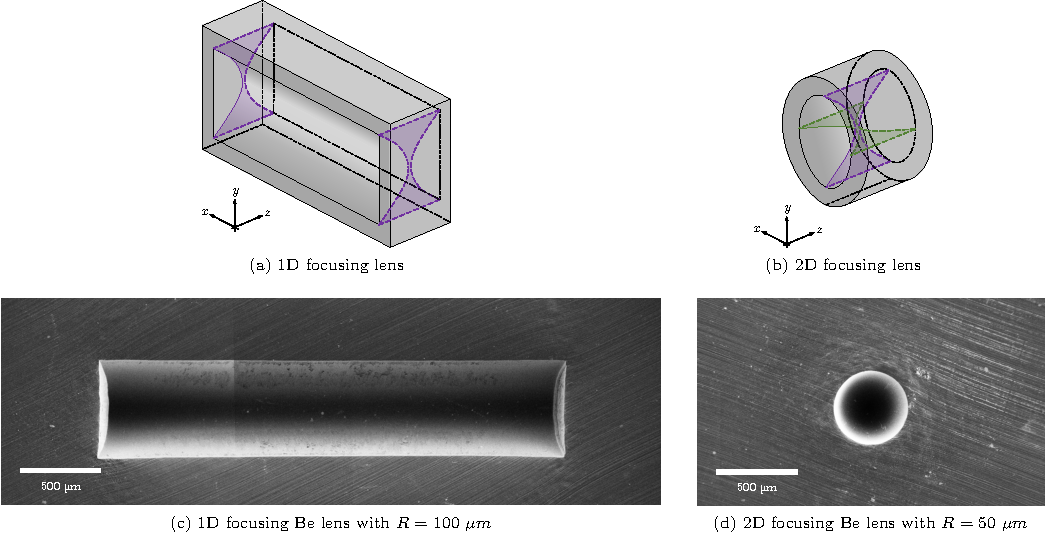
\includegraphics[width=.8\linewidth]{figures/ch03/1D2D.pdf}}
    \caption[1D and 2D focusing X-ray lenses]{1D (left) and 2D focusing (right) X-ray lenses. The top row shows a 3D rendering of such lenses with emphasis on the parabolic profile - shaded in purple is the vertical profile and in green, the horizontal profile. Bottom row shows scanning electron microscope (SEM) images of two Be lenses. Due to the limited field of view, image (c) is stitched, which explains the colour discontinuation on the left side of the image.} 
    \label{fig:1D2D_lenses}
\end{figure}

\begin{figure}[t]
    \centering
    {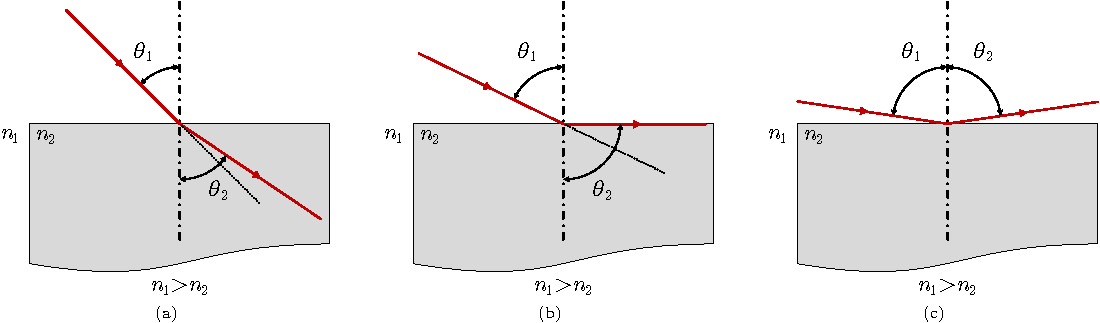
\includegraphics[width=0.7\linewidth]{figures/ch03/reflection_refraction.pdf}}
    \caption[Refraction and total external reflection in the X-ray regime]{Refraction and total external reflection in the X-ray regime.}
    \label{fig:reflection_refraction}
\end{figure}

From a simplistic point of view, the choice of material for an X-ray lens is guided by maximising the $\delta/\beta$ ratio for a given energy. This means choosing a material that will maximise refraction and minimise absorption within the lens [\cite{Serebrennikov2016, Roth2017}]. On a further step, knowledge about the material inner structure is also very relevant and minimising small angle scattering from the lenses, speckle formation and unwanted diffraction becomes relevant [\cite{Roth2014,Chubar2020,Lyatun2020}]. Ultimately, the choice of material is also connected to the the manufacturing process of the lenses. Commonly\footnote{A more broad overview on fabrication processes used for refractive X-ray lenses and materials is presented in Table~I from the supplementary materials in [\cite{Roth2017}].} used materials are aluminium and beryllium, which are usually associated with pressed lenses [\cite{refBe,refAl}]; Nickel and SU-8 polymer for deep X-ray lithography and LIGA [\cite{refLIGA}]; SU-8 and other polymeric materials are also associated with 3D printed lenses [\cite{ref3Dprinted}]; Silicon and glassy carbon for lithography and dry etching [\cite{refLithoLens}]; and more recently, diamond and glassy carbon for laser ablated lenses [\cite{refLaserLens}]. Figure~\ref{fig:refractive_index} shows $\delta$, $\beta$ and the ratio $\delta/\beta$ for energies ranging from 5~keV to 100~keV for aluminium, beryllium, diamond and SU-8. 

\begin{figure}[t]
    \centering
    {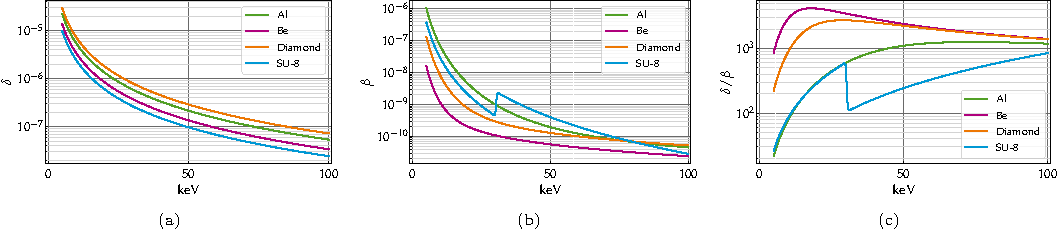
\includegraphics[width=1\linewidth]{figures/ch03/n_lens.pdf}}
    \caption[Index of refraction for common lens materials]{(a) refraction index decrement, (b) absorption index and (c) the $\delta/\beta$ ratio for energies ranging from 5~keV to 100~keV for aluminium, beryllium, diamond and SU-8. Figures obtained using the \textit{xraylib} library [\cite{Brunetti2004, Schoonjans2011}].}
    \label{fig:refractive_index}
\end{figure}


%-------------------------------------------------------------------------
%-------------------------------------------------------------------------
\subsection{CRL anatomy}\label{sec:CRL_anatomy}
%-------------------------------------------------------------------------
%-------------------------------------------------------------------------

\begin{figure}[t]
    \centering
    {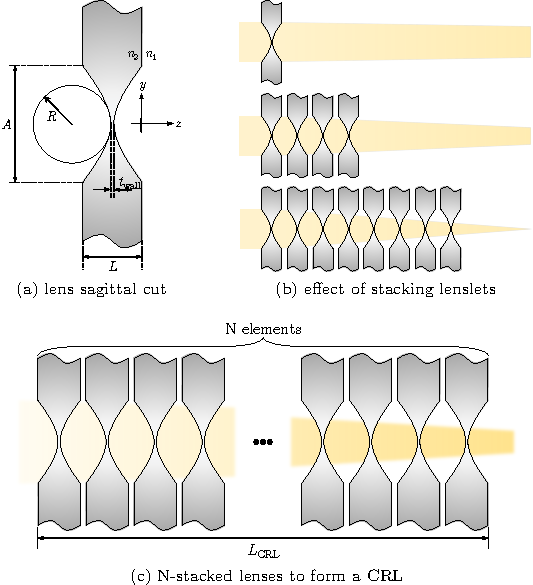
\includegraphics[width=0.5\linewidth]{figures/ch03/anatomy.pdf}}
    \caption[CRL anatomy]{(a) Sagittal cut of an X-ray lens showing its main geometrical parameters. This concave lens focuses X-rays in the $y$-direction if $n_1>n_2$. (b) A single X-ray lens refracts very weakly. To overcome this drawback - pointed out as early as the late 1940s [\cite{Kirkpatrick1948}] - lenses are usually stacked, hence "compound" in compound refractive lenses. (c) N-stacked lenses to form a CRL.}
    \label{fig:CRLs}
\end{figure}

Ideal parabolic X-ray lenses\footnote{Throughout this work, a single X-ray lens will be called a lenslet and two or more stacked lenses are referred to as compound refractive lens (CRL).} are usually defined by a small set of parameters as shown in Fig.~\ref{fig:CRLs}(a). These are: a) material, which, in conjunction with the operation energy defines the complex index of refraction $n$; b) apex radius of curvature ($R_x$ and $R_y$ for horizontal and vertical radii\footnote{For a 1D focusing lens, one of the radii goes to infinity on the non-curved surface. For a 2D focusing lens, the manufacturing goal is generally to produce lenses with $R_y=R_y=R$ to avoid astigmatism.}, respectively); c) lens thickness ($L$) or geometrical aperture ($A$); and d) distance between the apices of the parabolas ($\text{t}_{\text{wall}}$)\footnote{The web thickness ($\text{t}_{\text{wall}}$) is directly linked to the absorption and transmission of a X-ray lens, having no useful optical function. It should be kept as small as possible as to minimise absorption but as thick as necessary as to maintain the lenslet mechanical integrity. The exaggerated thinning of the web thickness leads to the risk or breaking the lens in brittle materials and shape deformation in ductile materials, deteriorating the lenslet performance [\cite{Lengeler1998}].}.

Firstly, one should start by defining the optical power $F=f^{-1}$ of a single refracting surface of radius $R$, where $f$ is its focal length. With the X-ray beam moving along the positive $z$-direction on Fig.~\ref{fig:CRLs}, the refracting power of the vacuum/lens interface is given by:
\begin{equation}\label{eq:Focus_simple}
    F\equiv\frac{1}{f}=\frac{n_2-n_1}{-R}=\frac{\delta}{R}.
\end{equation}{}
Eq.~\ref{eq:Focus_simple} considers only the real part of the indices of refraction as this is the part that governs the focusing effect of the lenses. As illustrated by Fig.~\ref{fig:CRLs}(a), lenses are typically formed by two refracting surfaces of nominally the same radii. From paraxial optics, the total optical power of refracting surfaces in intimate contact is the sum of their powers. The same is valid for the cases where the distance between them can be ignored. Typical materials used for X-ray lenses have $10^{-7}\leq\delta\leq10^{-3}$ for their usual application energies [\cite{Serebrennikov2016}]. To overcome the weak refraction of a single element, several X-ray lenses are stacked [\cite{Tomie1994, Snigirev1996}]. Still, under the assumption of thin elements:
\begin{equation}\label{eq:CRL_classic}
    f_{\text{thin}\text{~CRL}} = \frac{R}{2N\delta},
\end{equation}{}
where the $2N$ comes from stacking $N$ lenslets with two refracting surfaces each, as shown in Fig.~\ref{fig:CRLs}(b). A correction factor can be added to Eq.~\ref{eq:CRL_classic} in order to account for the thick-element nature of the CRL, as proposed in [\cite{Kohn2003}]. The corrected focal length for a thick CRL is given by:
\begin{equation}\label{eq:CRL}
        f_{\text{CRL}} = \frac{R}{2N\delta}+\frac{L_{\text{CRL}}}{6}.
\end{equation}{}
This focal distance is taken from the middle of the CRL and $L_{\text{CRL}}$ is the CRL longitudinal size, that is, distance from the front surface of the first optical element to the back surface of the last lens - cf. Fig.~\ref{fig:CRLs}(c). The number of lenslets stacked in a CRL is mainly limited by absorption of the X-rays propagating within the lenses. 
\begin{figure}[t]
    \centering
    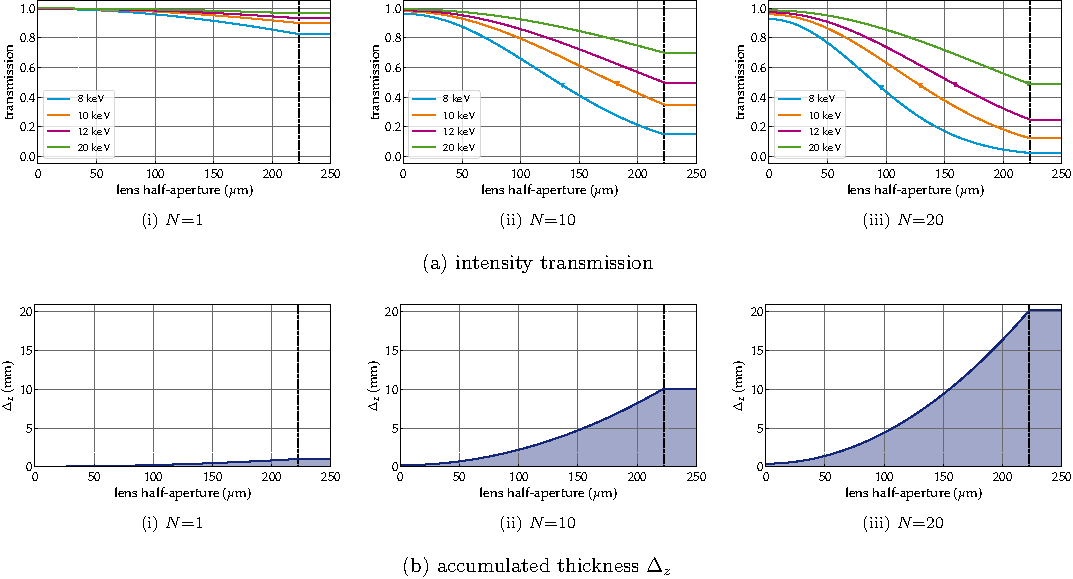
\includegraphics[width=1\linewidth]{figures/ch03/Aeff.pdf}
    \caption[Intensity transmission and accumulated thickness profile of CRLs]{(a) Normalised intensity transmission and (b) accumulated profile thickness for a CRL composed of ($\mathrm{i}$) 1, ($\mathrm{ii}$) 10 and ($\mathrm{iii}$) 20 2D-beryllium lenses with nominal radius $R=50~\mu\text{m}$, geometric aperture $A_{\diameter}=445~\mu\text{m}$ and $t_\text{wall}=20~\mu$m at different photon energies (for the intensity profiles). Vertical dashed line represents the lens geometrical half-aperture. The triangles in (a) indicate the full width at half maximum (fwhm) for the cases where this value lies within the geometrical aperture.}
    \label{fig:EffectiveAperure}
\end{figure}
Another important parameter for optical design is the lens geometrical aperture $A$, as it provides an upper bound for the numerical aperture of the system and, ultimately, to the theoretical optical resolving power. Assuming a parabolic profile of the refracting surface, the lens geometrical aperture can be calculated as:
\begin{equation}\label{eq:A}
    A = 2\sqrt{(L-\text{t}_\text{wall})R},
\end{equation}{}
where $L$ is the lenslet thickness and $\text{t}_\text{wall}$ is the distance between the apices of the parabolas, commonly referred to as web thickness. For a 1D-focusing lenslet, the aperture related to the uncurved surface is limited only by manufacturing constraints and not the intrinsic lens parameters. Depending on the process used for lens production, it is convenient to isolate $L$ in Eq.~\ref{eq:A}:
\begin{equation}\label{eq:L}
    L = \frac{A^2}{4R}+\text{t}_\text{wall}.
\end{equation}{}
It is clear from Eqs.~\ref{eq:A} and \ref{eq:L} that for a parabolic surface, $A$ and $L$ are intertwined. More often than not, the maximum aperture $A$ is limited by the absorption from the lens thickness on the edge of the parabolic surface (lens active area). The geometrical aperture defined in Eq.~\ref{eq:A} is greater than or equal to the \textit{effective} lens aperture\footnote{There are several reported ways of defining the \textit{effective} lens aperture - [\cite{Kohn2017}] discusses and compares some of the different definitions. } as indicated by [\cite{Kohn2017}]. Figure~\ref{fig:EffectiveAperure} shows the transmitted intensity profile of a CRL composed of a different number of 2D-beryllium lenses with nominal radius $R=50~\mu\mathrm{m}$ and circular geometric aperture $A_{\diameter}=445~ \mu\mathrm{m}$ at several energies. Unlike visible optics, where the transmitted intensity profile within the aperture, closely follows that of the illumination, the transmitted profile through a (stack of) X-ray lens(es) has strong absorption towards the edge, which defines the CRL as an apodised optical system.

% Note to myself: the critical angle limitation on the parabolic profile is not a real concern... aperture get's so large, that it makes no physically sense. Absorption is more pronounced. 

\begin{figure}[t]
    \centering
    {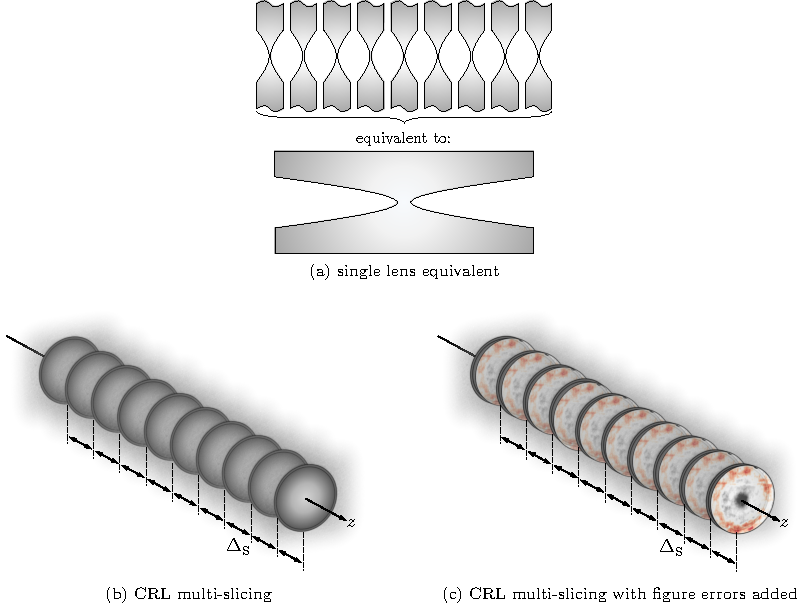
\includegraphics[width=0.8\linewidth]{figures/ch03/models.pdf}}
    \caption[Hierarchical CRL representation]{Hierarchical depiction of the CRL. (a) illustrates a single thin element equivalent of several lenslets. This representation accounts for net refraction and absorption in one transmission element but ignores intra-lens spacing. (b) multi-slice representation of a CRL. Here each lens of the stack is represented individually by one transmission element. Those are separated by a drift space corresponding to the typical distance between elements ($\Delta\text{s}$). (c) Not only can the CRL be represented as a series of thin elements separated by drift spaces, but also figure errors can be added. They are placed directly after the thin element representing a single X-ray lens.}
    \label{fig:models}
\end{figure}


\clearpage
%-------------------------------------------------------------------------
%-------------------------------------------------------------------------
\subsection{CRL modelling}\label{sec:CRL_modelling}
%-------------------------------------------------------------------------
%-------------------------------------------------------------------------

%-------------------------------------------------------------------------
%-------------------------------------------------------------------------
\subsubsection*{Ideal thin lens and single lens equivalent}\addcontentsline{toc}{subsubsection}{-- Ideal thin lens and single lens equivalent}
%-------------------------------------------------------------------------
%-------------------------------------------------------------------------

At any point inside the geometric aperture of a single paraboloidal X-ray lens, the projected thickness $\Delta_z$ can be calculated as:
\begin{equation}\label{eq:ProjecThick}
    \Delta_z(x,y) = 
     \begin{cases}
      \cfrac{x^2}{R_x}+\cfrac{y^2}{R_y}+\text{t}_\text{wall}, &\quad\forall~(x,y) \in A,\\
      L, &\quad\text{otherwise}.
     \end{cases}
\end{equation}
If the lens being modelled is a 1D focusing element, that is a cylinder with parabolic section, one of the radii goes to infinity to account for the non-curved surface. The geometric aperture in this direction is not given by Eq.~\ref{eq:A}, but arbitrarily chosen (cf. Fig.~\ref{fig:1D2D_lenses}). Eq.~\ref{eq:ProjecThick} can be substituted into Eqs.~\ref{eq:aux_funcs_transa} and \ref{eq:aux_funcs_transb} to retrieve the complex transmission element expression for an X-ray lens:
\begin{eqnarray}\label{eq:TE_singlelens} % https://tex.stackexchange.com/questions/74129/piecewise-function
    \mathrm{T}_{\text{single lens}}(\Delta_z)~\bullet =
    \exp{\bigg(-\frac{2\pi}{\lambda}\beta\Delta_z \bigg)}
    \times\exp{\bigg(-i\frac{2\pi}{\lambda}\delta\Delta_z \bigg)} \bullet.
\end{eqnarray}{}
Eq.~\ref{eq:TE_singlelens}, the single lens model, accounts for the absorption (first exponential) and phase shift (second exponential) \footnote{The constant phase shift induced by $t_\text{wall}$ in Eq.~\ref{eq:TE_singlelens} (cf. Eq.~\ref{eq:ProjecThick}) can often be disregarded, as it impinges a constant phase to the wave-field.}. The complex transmission representing a CRL composed of $N$ elements is, thus, represented by:
\begin{equation}\label{eq:TE_CRL}
    \mathrm{T}_{\text{CRL}}(\Delta_z)~\bullet = \big[\mathrm{T}_{\text{single lens}}(\Delta_z)\big]^{N} \bullet,
\end{equation}{}
which is equivalent to multiplying $\Delta_z$ by $N$ in Eq.~\ref{eq:TE_singlelens}. The model represented by Eq.~\ref{eq:TE_CRL} will be referred to as the single lens equivalent. This model represents a lens stack by a single transmission element with equivalent focal distance and the projected thickness of all the $N$ single lenses as shown in Fig.~\ref{fig:models}(a).

%-------------------------------------------------------------------------
%-------------------------------------------------------------------------
\subsubsection*{Multi-slicing representation}\addcontentsline{toc}{subsubsection}{-- Multi-slicing representation}
%-------------------------------------------------------------------------
%-------------------------------------------------------------------------

For a CRL composed of a very high number of lenslets, the single-lens equivalent approximation (Eq.~\ref{eq:TE_CRL}) may not be adequate to correctly represent such optical systems mainly due to the thick\footnote{In terms of optical element modelling.} nature of the stack  - evidenced by Eq.~\ref{eq:CRL}; and due to the progressive focusing inside the CRL [\cite{Schroer2005}] - exaggerated in Fig.~\ref{fig:CRLs}. For such cases, it is possible to adapt the multi-slicing (MS) techniques\footnote{cf. \textit{The Multi-slice approximation} in \S\ref{sec:thin_element}~-~\textit{\nameref{sec:thin_element}}.} for the calculation of the transmission of a wavefront through a CRL. Unlike the methods described by [\cite{Paganin2006}] and most recently, by [\cite{Li2017}] and [\cite{Munro2019}], where a single weakly-scattering optical element is sliced into several slabs, it is sufficient for most practical cases to break down a CRL into its lenses as shown in  Fig.~\ref{fig:models}(b). This can be justified by the fact that at their typical operation energy, the materials used for lens manufacturing have a very low $\delta$ [\cite{Serebrennikov2016}], rendering the individual lenslets a weak focusing element where the projection approximation holds [\cite{Protopopov1998}]. The complex transmission representation of a CRL based on the MS approach is given by:

\begin{equation}\label{eq:TE_CRL_MS}
    \mathrm{T}_{\text{CRL-MS}}(\Delta_z)~\bullet = \mathrm{T}_{\text{single lens}}(\Delta_z)\cdot\big[\mathcal{D}({\Delta}\text{s})\cdot\mathrm{T}_{\text{single lens}}(\Delta_z)\big]^{N-1}\bullet,
\end{equation}{}
where $\mathcal{D}({\Delta}\text{s})$ is the operator formulation of the Fresnel free-space propagation over a distance $\Delta\text{s}$ (distance between the centre of two adjacent lenses) - cf. Eqs.~\ref{eq:MS} and \ref{eq:Fresnel_operator}. 

Eq.~\ref{eq:TE_CRL_MS} represents a wavefront $\bullet$ modified by a single lens complex transmission $\mathrm{T}_{\text{single lens}}$, followed by free-space propagation $\mathcal{D}({\Delta}\text{s})$ over a distance $\Delta \text{s}$. The multiplication of the resulting electric field by the transmission element and subsequent free-space propagation is done $(N-1)$ times until the $N^{\text{th}}$ lens is reached and the last element of the lens stack is accounted for.

Optical imperfections measured with high spatial resolution can be readily converted into a transmission element by direct application of Eq.~\ref{eq:transmission_operator} to the height profile, provided it is a 2D map of the phase defects. In this case, the height profile will be the projected thickness of $\Delta_z(x,y)$ in the preceding equations. The MS model introduced earlier in this section can then be adapted to account for the phase errors of the individual lenses:
\begin{equation}\label{eq:TE_CRL_MS_ERR}
    \mathrm{T}_{\text{CRL-MS}}(\Delta_z)~\bullet = \mathrm{T}_{\text{imperfect lens}}(\Delta_z)\cdot\big[\mathcal{D}({\Delta}\text{s})\cdot\mathrm{T}_{\text{imperfect lens}}(\Delta_z)\big]^{N-1}\bullet,
\end{equation}{}
with:
\begin{equation}\label{eq:TE_CRL_single_ERR}
    \mathrm{T}_{\text{imperfect lens}}(\Delta_z) = \mathrm{T}_{\text{figure errors}}(\Delta_z)\cdot\mathrm{T}_{\text{single lens}}(\Delta_z).
\end{equation}{}
This extended version of the MS model is shown in Fig.~\ref{fig:models}(c). In fact, the modelling of optical elements by means of  Eq.~\ref{eq:TE_CRL_MS_ERR} allows for the description of inhomogenities in the index of refraction within the lens as differences in material density and grain size [\cite{Lyatun2020}], inclusions and voids [\cite{Roth2014}], and even include effects of diffuse scattering/SAXS for a 2D map with very high spatial resolution [\cite{Paganin2019}].

%-------------------------------------------------------------------------
%-------------------------------------------------------------------------
\subsection{CRL performance}\label{sec:CRL_performance}
%-------------------------------------------------------------------------
%-------------------------------------------------------------------------

%-------------------------------------------------------------------------
%-------------------------------------------------------------------------
\subsubsection*{Diffraction limited focal spot}\addcontentsline{toc}{subsubsection}{-- Diffraction limited focal spot}
%-------------------------------------------------------------------------
%-------------------------------------------------------------------------

Even an ideal and aberration-free finite optical element is not able to image a point-source to a point-like image. Limiting the extent of the focusing element by defining an aperture will induce diffraction effects on the wavefront and these will limit the smallest reachable focus spot size. The normalised response of the optical system to this point-like source input is called the point-spread-function (PSF). For a system with circular aperture and uniform amplitude across the exit pupil, the intensity of such focused beam at the image plane is proportional to a squared first-order Bessel function of the first kind (Airy pattern). The FWHM of the central cone is given by:
\begin{align}\label{eq:PSF}
    d = 1.22\lambda (1-M)\frac{f_{\text{CRL}}}{A},
\end{align}{}
where the $M$ is the magnification of the system, which goes to zero for a plane wave or a very distant source. Systems with nonuniform illumination at the pupil exit, in the case of the CRLs, an apodised systems approaching a Gaussian illumination, may present a different PSF shape depending on the truncation imposed by the aperture. A very weakly truncated focusing system will have a Gaussian-shaped focal spot as little to no cropping occurs and therefore diffraction effects can be neglected. Increasing the truncation of the beam enhances diffraction effects from the geometric aperture. A strongly truncated focusing system will have a PSF that resembles the diffraction pattern in the far-field associated with the aperture of the system\footnote{The far-field diffraction pattern of a circular aperture is a squared first-order Bessel function profile while a square aperture will produce a 2D sinc-squared pattern [\cite{Guasti1993}].} [\cite{Mahajan1986}]. 
% where the $M$ is the magnification of the system, which goes to zero for a plane wave or a very distant source. Systems with nonuniform illumination at the pupil exit, in the case of the CRLs, an apodised systems approaching a Gaussian illumination, may present a different PSF shape depending on the truncation imposed by the aperture  (see Fig.~\ref{fig:PSF}). A very weakly truncated focusing system will have a Gaussian-shaped focal spot as little to no cropping occurs and therefore diffraction effects can be neglected. Increasing the truncation of the beam enhances diffraction effects from the geometric aperture. A strongly truncated focusing system will have a PSF that resembles the diffraction pattern in the far-field associated with the aperture of the system\footnote{The far-field diffraction pattern of a circular aperture is a squared first-order Bessel function profile while a square aperture will produce a 2D sinc-squared pattern [\cite{Guasti1993}].} [\cite{Mahajan1986}]. 
%\todo{Figure with 2 graphs side by side: transmission (like Fig \ref{fig:EffectiveAperure}) and the horizontal cut of the PSF. 4 curves: 100\% transmisson on the edge of A, 75\%, 1$/e^2$ and 0}


%-------------------------------------------------------------------------
%-------------------------------------------------------------------------
\subsubsection*{Tolerance conditions for aberrations}\addcontentsline{toc}{subsubsection}{-- Tolerance conditions for aberrations}
%-------------------------------------------------------------------------
%-------------------------------------------------------------------------

Introducing errors to the optical system will reduce the peak intensity in the PSF [\cite[\textit{\S8.2}]{Mahajan2011}]. The ratio between the peak intensities of the aberrated- and non-aberrated PSF of a system with the same aperture and focal length is referred to as the Strehl ratio - cf. \S9.1.3 in [\cite{born_wolf1999}]. The optical aberrations on the exit pupil of an optical system can be described by the aberration function $\Phi(x,y)$, with the dimension of metres, which represents any deviation in shape from an ideal profile. For small aberration values, the Strehl ratio can be approximated\footnote{Eqs.~\ref{eq:Strehl}-\ref{eq:Mahajan} were obtained using a fully-coherent illumination of the optical system, however, defining the Strehl ratio as the ratio between the peak intensities of the aberrated- and non-aberrated optical under study transcends the nature of the illumination. A more complete derivation of the Strehl ratio (Eq.~\ref{eq:Strehl}) can be found in \S9.1.3 - \textit{A relation between the intensity and the average deformation of wave-fronts} in [\cite{born_wolf1999}].} by:
\begin{equation}\label{eq:Strehl}
    S_{\text{ratio a}}=\frac{I_{\text{aberrated}}}{I_{\text{aberration free}}}\approx1-\bigg(\frac{2\pi}{\lambda}\bigg)^2\Delta\Phi^2,
\end{equation}{}
where $\Delta\Phi$ is the standard deviation of the aberration function $\Phi(x,y)$. An important consequence of Eq.~\ref{eq:Strehl} is that the reduction in the peak intensity on the focal plane does not depend on the type of aberration nor the focal length of the optical system, but on its standard deviation across the exit pupil of the optical system [\cite{born_wolf1999}]. Alternative expressions to Eq.~\ref{eq:Strehl} are available in \S8.3 of [\cite{Mahajan2011}], namely:
\begin{align}\label{eq:Marechal}
    S_{\text{ratio b}}\approx\bigg[1-\bigg(\frac{2\pi}{\lambda}\bigg)^2\frac{\Delta\Phi^2}{2}\bigg]^2,
\end{align}
known as the Mar\'echal expression and:
\begin{align}\label{eq:Mahajan}
    S_{\text{ratio c}}\approx\exp{\bigg[- \bigg(\frac{2\pi}{\lambda}\bigg)^2\Delta\Phi^2\bigg]},
\end{align}
an empiric expression that fits better numerical results [\cite{Wetherell1980}]. However, for strong aberrations, there is no simple analytic expression to describe the relation between the Strehl ratio and the standard deviation of the aberration function $\Phi(x,y)$ [\cite{Kessler81}]. 

It is possible to define an arbitrary minimum acceptable value to the Strehl ratio when evaluating an optical element quality (tolerancing). This value depends on the final application and the desired performance. However, a value of $S_\text{ratio}\geq0.8$ is commonly found throughout literature as an indicator of a well-corrected optical system\footnote{This comes from historic reasons: both Rayleigh's $\lambda/4$ criterion for spherical aberrations (1879) and the extended Mar\'echal criterion for optical quality (1943) yield in a Strehl ratio of $\sim0.8$ [\cite{born_wolf1999}].}. Inserting $S_\text{ratio}\geq0.8$ in Eq.~\ref{eq:Strehl}, one obtains:
\begin{equation}\label{eq:MarechalCriterion}
    |\Delta\Phi|\leq\frac{\lambda}{14},
\end{equation}{}
which is known as the Mar\'echal criterion for optical quality. Equations~\ref{eq:Marechal}~and~\ref{eq:Mahajan} give similar limits: $\lambda/13.67$ and $\lambda/13.30$, respectively. In order to apply  Eq.~\ref{eq:MarechalCriterion} to the case of an X-ray lens, one makes use of Eq.~\ref{eq:aux_funcs_transb} with $\Delta\phi =\frac{2\pi}{\lambda}\delta\sigma_z=\frac{2\pi}{\lambda}|\Delta\Phi|$, where $\Delta\phi$ is the  standard deviation of the phase, and replaces the projected thickness\footnote{cf. \textit{The projection approximation} in \S\ref{sec:thin_element}~-~\textit{\nameref{sec:thin_element}}.} $\Delta_z$ with the standard deviation of the projected figure error $\sigma_z$:
\begin{align}\label{eq:ThickLim}
    \sigma_z &\leq \frac{\lambda}{14\delta}.
\end{align}{}
Equation \ref{eq:ThickLim} gives an upper limit to the standard deviation of accumulated figure errors for X-ray lenses in order to comply with the Mar\'echal criterion of tolerable wavefront aberrations, or in other words, to sustain a $S_\text{ratio}\geq0.8$. For a more complete discussion on the aberrated PSF, Strehl ratio and tolerance conditions for primary aberrations, refer to \S9 from [\cite{born_wolf1999}] and \S8 from [\cite{Mahajan2011}]. The limitations and applicability of the Maréchal criterion is presented in [\cite{Ross2009}].

%-------------------------------------------------------------------------
%-------------------------------------------------------------------------
\subsubsection*{Chromatic aberrations}\addcontentsline{toc}{subsubsection}{-- Chromatic aberrations}
%-------------------------------------------------------------------------
%-------------------------------------------------------------------------

The optical properties of the X-ray lenses are strongly dependent on the wavelength as both $\delta$ and $\beta$ have an energy dependency. This causes chromatic aberrations and limitations on the optical performance of the CRL under an X-ray beam with finite bandwidth. X-ray lenses in storage rings are often used after a monochromator - eg. Si(111) with $\Delta \text{E}/\text{E}\approx10^{-4}$. Under such conditions the effects of the beam bandwidth can often be neglected, which is not the case for the white- or pink-beam from bending magnets and undulators [\cite{Seiboth2014}]. The chromaticity of X-ray lenses can, however, be used favourably for X-ray harmonic rejection from insertion devices and coarse X-ray spectrum filtering [\cite{Vaughan2011, Polikarpov2014}]. $\blacksquare$
\addcontentsline{toc}{section}{References}
\printbibliography[heading=subbibliography]
\end{refsection}


